\documentclass[a4paper,12pt]{article}

\usepackage[utf8]{inputenc}
\usepackage{graphicx}
\usepackage{amsmath}
\usepackage{amsfonts}
\usepackage{geometry}
\geometry{a4paper, left=1in, right=1in, top=1in, bottom=1in}
\usepackage{hyperref}
\usepackage{fancyhdr}
\usepackage{float}

% Titre du document
\title{Rapport Technique sur le Projet "Thunder Game"}
\author{Taleb Ahmed 000575310}
\date{\today}

% En-têtes de page
\pagestyle{fancy}
\fancyhf{}
\fancyhead[L]{Thunder Game}
\fancyhead[C]{Rapport Technique}
\fancyhead[R]{\thepage}

\begin{document}
	
	% Titre
	\maketitle
	
	\begin{abstract}
		Ce document présente un rapport du projet \textbf{Thunder Game}. Le jeu, développé en utilisant le langage de programmation Processing, implique des mécanismes de jeu liés à un personnage contrôlé par l'utilisateur qui doit éviter des éclairs dans un environnement dynamique. Le rapport aborde la structure du code, l'architecture du jeu, et les principales fonctionnalités implémentées.
	\end{abstract}
	
	\newpage
	\tableofcontents
	\newpage
	
	\section{Introduction}
	
	\subsection{Objectifs du Projet}
	\noindent L'objectif principal du projet \textbf{Thunder Game} est de créer un jeu interactif où le joueur contrôle un personnage nommé Bob, qui doit éviter des éclairs en mouvement dans un environnement. Le jeu se compose de différents niveaux de difficulté et permet de suivre les scores.
	
	\subsection{Technologies Utilisées}
	\noindent Le projet a été développé en utilisant le langage de programmation \texttt{Processing} pour le rendu graphique et la gestion des entrées utilisateur. La gestion des scores et des niveaux se fait via une structure de données qui sauvegarde les informations dans un fichier texte.
	
	\newpage
	\section{Architecture du Jeu}
	
	\subsection{Classes Principales}
	\noindent Le jeu est constitué de plusieurs classes qui gèrent différentes fonctionnalités du jeu. Voici une brève description des classes principales :
	
	\begin{itemize}
		\item \textbf{Bob}: Représente le personnage contrôlé par le joueur. Il peut se déplacer à l'écran et interagir avec les éclairs.
		\item \textbf{Strike}: Représente un éclair. Il gère le mouvement, l'apparition et les ramifications de l'éclair.
		\item \textbf{Level}: Définit les paramètres de chaque niveau, comme la vitesse des éclairs et le nombre maximal d'éclairs à l'écran.
		\item \textbf{Leaderboard}: Gère les scores du jeu, en enregistrant les meilleurs scores dans un fichier.
		\item \textbf{ManageScore}: Gère le score du joueur, en le mettant à jour à chaque action.
		\item \textbf{ManageDisplay}: Gère l'affichage du jeu, y compris le fond, les nuages, le sol et les éléments UI comme le score et le niveau.
		\item \textbf{ManageStrike}: Gère la création, le mouvement et la collision des éclairs.
	\end{itemize}
	
	\subsection{Encapsulation}
	\noindent Des notions d'encapsulation ont été intégrées au projet afin de respecter les bonnes pratiques de la programmation orientée objet. Les données membres des différentes classes (comme le score, les niveaux ou les éclairs) sont gérées via des méthodes d'accès (\textit{getters} et \textit{setters}) lorsque nécessaire, ce qui permet de mieux contrôler la modification des attributs internes et de garantir l'intégrité de l'état des objets. Cela favorise également une meilleure lisibilité, modularité et maintenabilité du code.
	
	\newpage
	\section{Fonctionnalités du Jeu}
	
	\subsection{Mécanismes de Jeu}
	\noindent Le jeu commence au niveau \textbf{Basic} avec Bob sur l'écran, et des éclairs commencent à apparaître. L'objectif est de contrôler Bob horizontalement à l'aide des flèches gauche et droite pour éviter les éclairs qui tombent verticalement, tout en accumulant des points. Le joueur doit réagir rapidement pour déplacer Bob et éviter les éclairs qui descendent du haut de l'écran.
	
	\noindent À chaque niveau, les éclairs deviennent plus rapides, et le nombre d'éclairs actifs à l'écran augmente. De plus, à mesure que le joueur progresse dans les niveaux, la vitesse de Bob diminue et son inertie augmente, ce qui rend les mouvements plus difficiles à contrôler. Ces ajustements visent à augmenter la difficulté du jeu à chaque niveau et à offrir un défi croissant au joueur.
	
	\noindent Le score augmente chaque fois qu'un éclair est évité avec succès. Lorsqu'un éclair touche Bob, le score est réinitialisé à zéro, et le joueur doit recommencer à accumuler des points. Chaque niveau offre ainsi une progression dynamique, avec une difficulté croissante et un score de plus en plus difficile à maintenir.
	
	\subsection{Gestion des Niveaux}
	\noindent Il y a trois niveaux de difficulté dans le jeu :
	
	\begin{itemize}
		\item \textbf{Basic}: Le niveau le plus facile, avec une vitesse d'éclairs faible, un seul éclair actif à la fois et une grande distance de ralentissement pour Bob.
		\item \textbf{Medium}: Niveau 2-Medium, avec des éclairs plus rapides, jusqu'à deux éclairs actifs à la fois, et un ralentissement sur une distance plus courte pour Bob.
		\item \textbf{Expert}: Niveau 3-Expert, avec des éclairs très rapides, trois éclairs actifs en même temps, et un ralentissement encore plus court pour Bob.
	\end{itemize}
	
	\subsection{Système de Scores}
	\noindent Les scores sont enregistrés dans un fichier texte et affichés à l'écran. Le joueur peut voir son score actuel et son meilleur score. Un classement des meilleurs scores est également disponible à partir d'un fichier enregistré.
	
	\newpage
	\section{Tests et Validation}
	
	\subsection{Tests Fonctionnels}
	Des tests fonctionnels ont été effectués pour s'assurer que les différents niveaux de difficulté sont correctement implémentés, que les scores sont bien sauvegardés et affichés, et que l'expérience de jeu est fluide.
	
	\section{Fonctionnement}
	
	\subsection{Déroulement de la partie}
	
	Lorsque vous lancez une partie, le premier écran vous permet d’introduire votre nom.
	\begin{figure}[H]
		\centering
		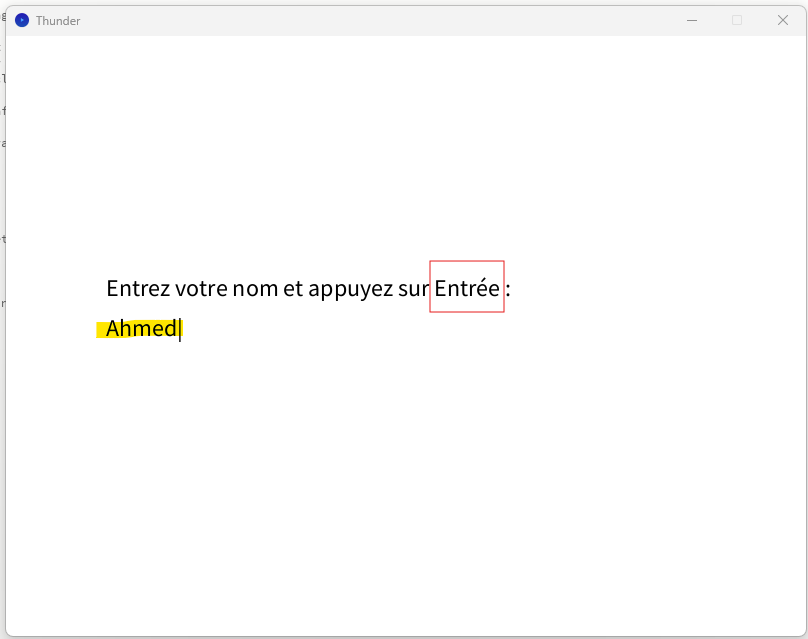
\includegraphics[width=0.5\textwidth]{1.png}
		\caption{Écran de saisie du nom du joueur}
	\end{figure}
	
	Lorsque celui-ci est introduit et que vous appuyez sur la touche \texttt{Entrée}, la partie se lance.
	\begin{figure}[H]
		\centering
		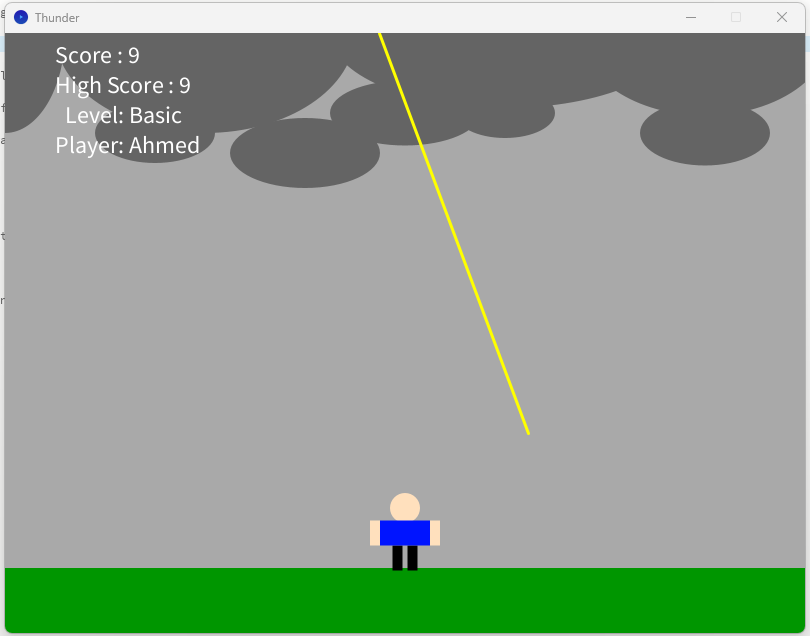
\includegraphics[width=0.5\textwidth]{2.png}
		\caption{Début de la partie après la saisie du nom}
	\end{figure}
	
	Vous pouvez changer de niveau en appuyant sur la touche \texttt{1} pour le niveau Basic, \texttt{2} pour Medium et \texttt{3} pour Expert.
	\begin{figure}[H]
		\centering
		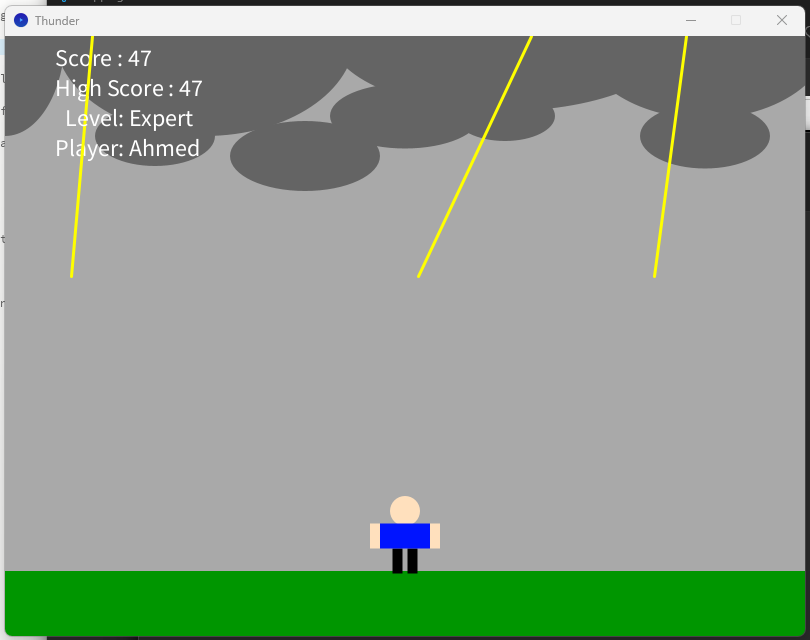
\includegraphics[width=0.5\textwidth]{4.png}
		\caption{Changement de niveau avec les touches 1, 2, 3}
	\end{figure}
	
	À tout moment de la partie, vous pouvez consulter le top 10 des meilleurs scores en appuyant sur la touche \texttt{Espace}. Cela met le jeu en pause.
	\begin{figure}[H]
		\centering
		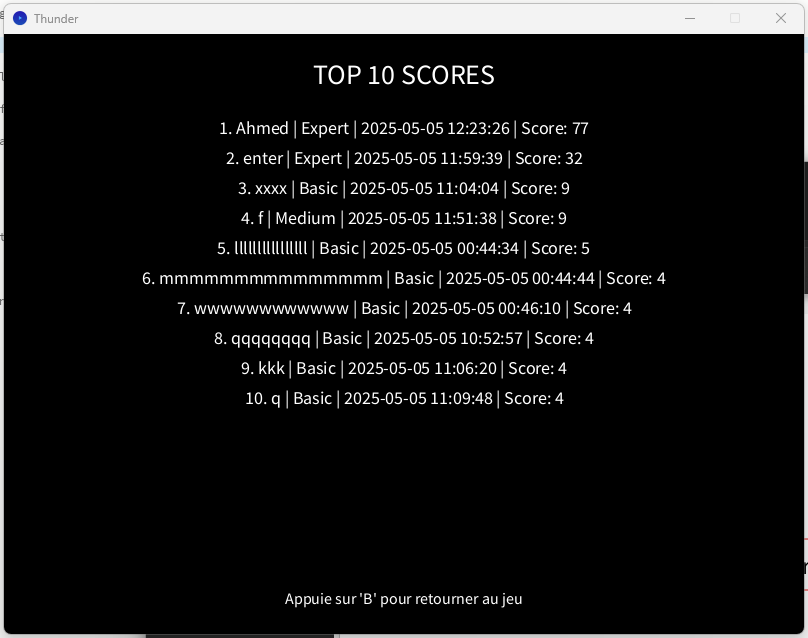
\includegraphics[width=0.5\textwidth]{3.png}
		\caption{Affichage du classement des meilleurs scores}
	\end{figure}
	
	Si vous souhaitez reprendre le jeu, vous pouvez quitter l’écran des meilleurs scores en appuyant sur la touche \texttt{B}.
	
	\noindent Enfin, si vous souhaitez quitter le jeu, appuyez sur la touche \texttt{Q}. Cette action permet de sauvegarder automatiquement votre meilleur score.
	
	\subsection{Limite du projet}
	\noindent Le mode Expert avec des éclairs ramifiés, prévu pour renforcer la difficulté du jeu, n’a pas pu être développé faute de temps. Cette fonctionnalité, bien que prévue initialement, reste une amélioration possible pour une version ultérieure du projet.
	
	\newpage
	\section{Conclusion}
	
	Le projet \textbf{Thunder Game} est un jeu simple mais dynamique, qui met en œuvre les concepts fondamentaux de la programmation orientée objet. Les principales difficultés rencontrées ont concerné l'aspect graphique du jeu. Certains éléments liés à l'affichage n'ont malheureusement pas pu être finalisés comme prévu, faute de temps. Enfin, le débogueur intégré à Processing 4.3 s’est révélé particulièrement utile, car il m’a permis de suivre pas à pas l’exécution du programme, d’identifier plus facilement l’origine des problèmes rencontrés et de les corriger efficacement.
	
\end{document}
